% fig06_bz_parity.tex — On-axis Bz: closed-form anchor vs GetDP FEM bridge.
% Compiled by the paper Makefile via `make figures` (pdflatex on the snippet).
%
% Data: Appendix D (TF magnet), Table "tab:app:mesh". On-axis Bz(0) [T]:
%   closed-form anchor solenoid_axis_bz(2e6,.5,.7,1.2) = 1.48265 T
%   GetDP 33k-node (3.5.0 Linux / 4.0.0 Apple silicon)  = 1.4817  T  (Delta=-0.064%)
%   GetDP 61k-node (3.5.0 Linux)                        = 1.4782  T  (Delta=-0.30%)
% Verify atoms solenoid_axis_bz / magnet_gate_b_peak (PR #1084 / #1095).
% A zoomed y-axis (1.475-1.485) makes the sub-percent gaps visible; the
% per-bar Delta annotations are the registered residuals.
%
% Manual single-shot compile (debug):
%   pdflatex -interaction=nonstopmode -halt-on-error fig06_bz_parity.tex
\documentclass[border=4pt]{standalone}
\usepackage{tikz}
\usepackage{pgfplots}
\pgfplotsset{compat=1.18}
\begin{document}
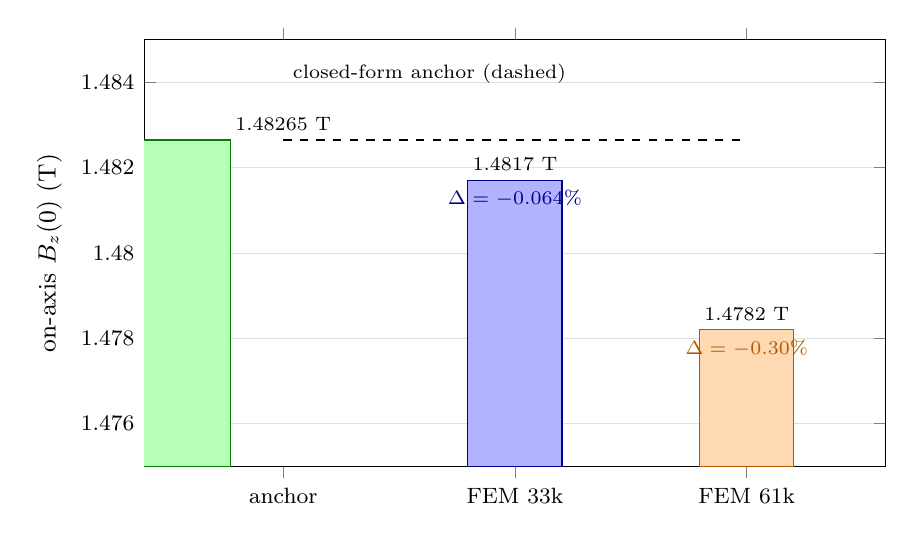
\begin{tikzpicture}
\begin{axis}[
  width=11cm, height=7cm,
  ybar,
  bar width=34pt,
  ymin=1.475, ymax=1.485,
  ylabel={on-axis $B_z(0)$ (T)},
  symbolic x coords={anchor, FEM 33k, FEM 61k},
  xtick={anchor, FEM 33k, FEM 61k},
  tick label style={font=\footnotesize},
  label style={font=\small},
  ymajorgrids,
  grid style={gray!25},
  enlarge x limits=0.30,
  /pgf/number format/.cd, fixed, precision=5,
]
% closed-form anchor (reference dashed line)
\addplot[draw=black,dashed,thick,sharp plot,update limits=false] coordinates {
  (anchor,1.48265) (FEM 61k,1.48265)
};
\addplot[draw=green!50!black,fill=green!28] coordinates {
  (anchor,1.48265)
};
\addplot+[draw=blue!55!black,fill=blue!30,bar shift=0pt] coordinates {
  (FEM 33k,1.4817)
};
\addplot+[draw=orange!70!black,fill=orange!30,bar shift=0pt] coordinates {
  (FEM 61k,1.4782)
};
% annotations
\node[font=\scriptsize,anchor=south] at (axis cs:anchor,1.48265)
  {1.48265 T};
\node[font=\scriptsize,anchor=south] at (axis cs:FEM 33k,1.4817)
  {1.4817 T};
\node[font=\scriptsize,anchor=north,text=blue!55!black] at (axis cs:FEM 33k,1.4817)
  {$\Delta=-0.064\%$};
\node[font=\scriptsize,anchor=south] at (axis cs:FEM 61k,1.4782)
  {1.4782 T};
\node[font=\scriptsize,anchor=north,text=orange!70!black] at (axis cs:FEM 61k,1.4782)
  {$\Delta=-0.30\%$};
\node[font=\scriptsize,text=black,anchor=west] at (axis cs:anchor,1.4842)
  {closed-form anchor (dashed)};
\end{axis}
\end{tikzpicture}
\end{document}
